\chapter{Propsed Work}
As the existing state of art model were for natural images, we trained the existing model on wireless capsule endoscopy dataset to check which kind of network is best suitable for the WCE images. after carefully studying the outputs of SOTA models, we reached a conclsion that the network having desne connections learns this images very well. Mean while we came across a reseach paper based on CycleCNN {\cite{CycleCNN}} to accomplish the task of image super resolution. we took CycleCNN as the base network and started the experimental work.
\section{CycleCNN}
Initially CycleCNN was proposed for unsupervised training method, we made relevant changes in the network to train it using supervised training method. The network architecture for the cycleCNN is shown in the Fig. \ref{fig:label6.1} and Fig. \ref{fig:label6.2}



\begin{figure}[H]
    \centering
    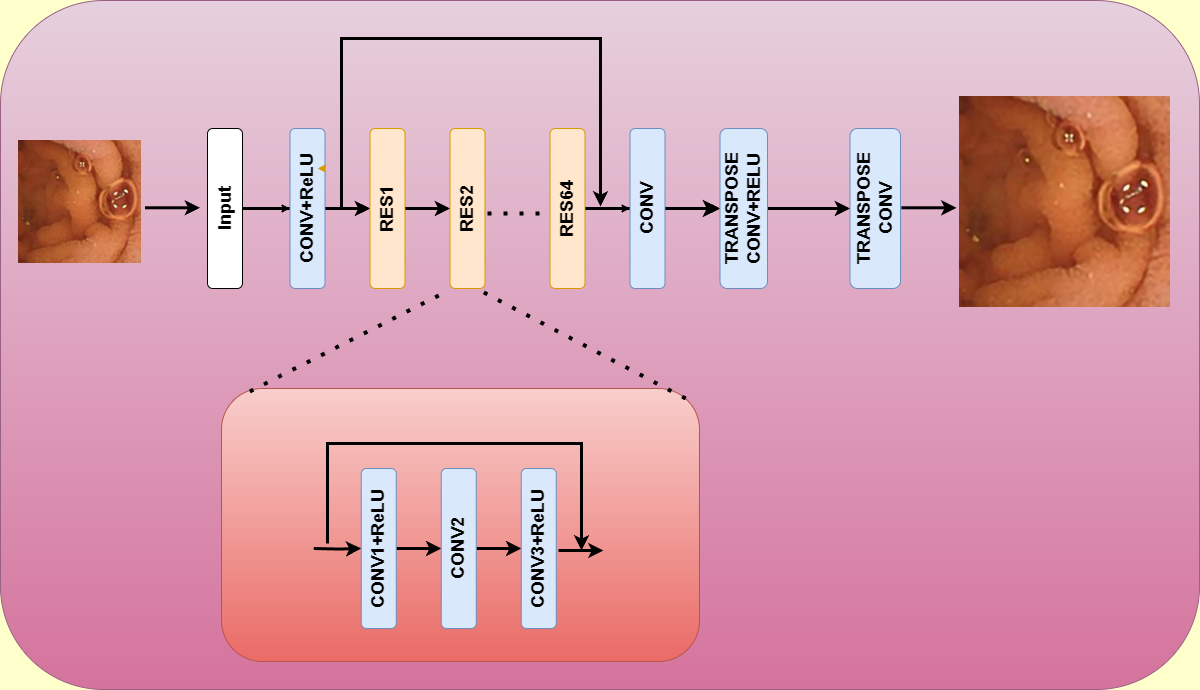
\includegraphics[totalheight=3.5in]{Chapter6/CycleCNN_UP.png}
    \caption[Upsampling Network of CycleCNN]{Upsampling Network of CycleCNN}
    \label{fig:label6.1}
\end{figure}

\begin{figure}[H]
    \centering
    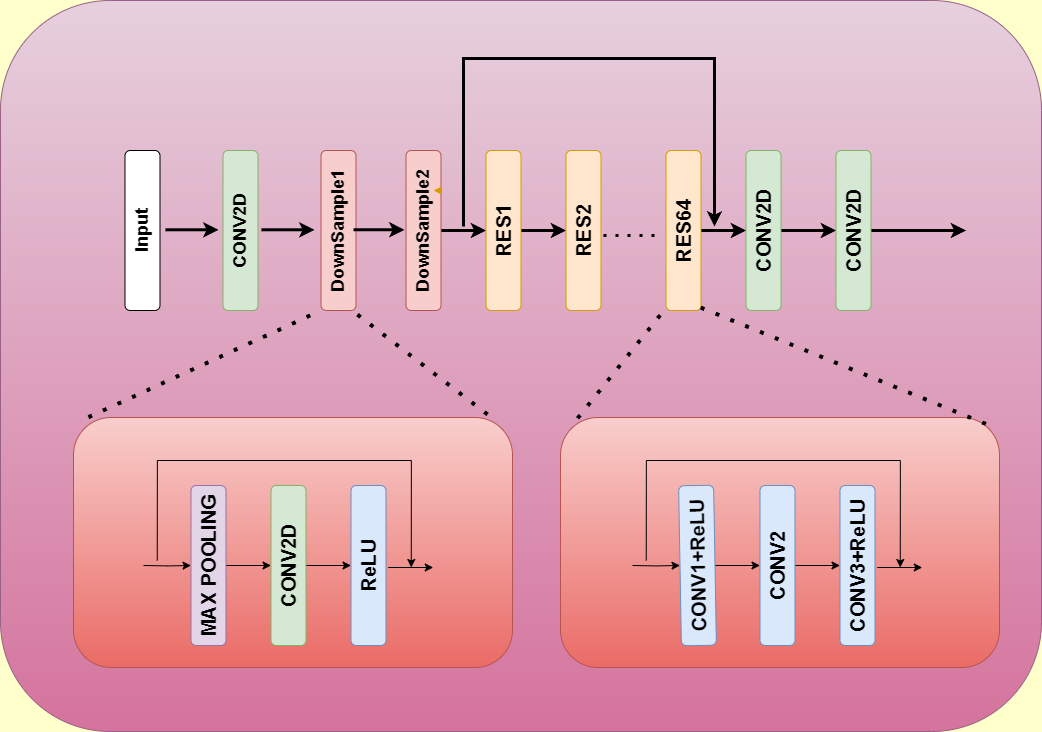
\includegraphics[totalheight=4.5in]{Chapter6/dd_1.png}
    \caption[Downsampling Network of CycleCNN.]{Downsampling Network of CycleCNN}
    \label{fig:label6.2}
\end{figure}
Where each convolution layer has 3x3 kernel size with stride 1 and padding 1, while the transpose convolution layer has kernel size 3x3 with stride 2 and padding 1. 
\subsection{CycleCNN-MSE}
The training of CycleCNN was performed on different loss functions. Firstly, it was trained on mean-squared error (MSE) loss. The same architecture was parallelly trained on cycle loss as well as MSE loss. The equations for MSE loss and Cycle loss is defined in equation \ref{eqn:mse} and \ref{eqn:cycle} respectively.

\begin{equation*}\label{eqn:mse}
{L_{MSE}} = \sum_{i=1}^{D}(x_{ti}-y_{ti})^2 \tag{5.1}\end{equation*}


\begin{equation*}
\label{eqn:cycle}
{L_{cyc}} = \frac{1}{N}\sum\limits_{i = 1}^N {\left( {{{\left\| {{G_2}({G_1}({x_{ti}})) - {x_{ti}}} \right\|}_2} + {{\left\| {{G_1}({G_2}({y_{ti}})) - {y_{ti}}} \right\|}_2}} \right)} \tag{5.2} \end{equation*}


The results for training on MSE loss as well as MSE and cycle loss are given the Fig 
\ref{fig:label7.1}

 

\section{Dense CycleCNN with GRL Block}
By comparing the State of art models, it is evident that the modalities of capsule endoscopy data was very well learnt by dense connections(DenseNet). Dense connections are able to capture the high frequency details which are important for our case. To improve the results obtained from CycleCNN we introduced dense connections in the model.Global Resudial Learning(GRL) block was also introduced to resolve the issue of gradinet vanishing and to stabalize the training. The GRL block is used to propogate the input directly at the end of the model.  The network architecture for this model is given in Fig. \ref{fig:label6.4} and Fig. \ref{fig:label6.6}

\begin{figure}[H]
    \centering
    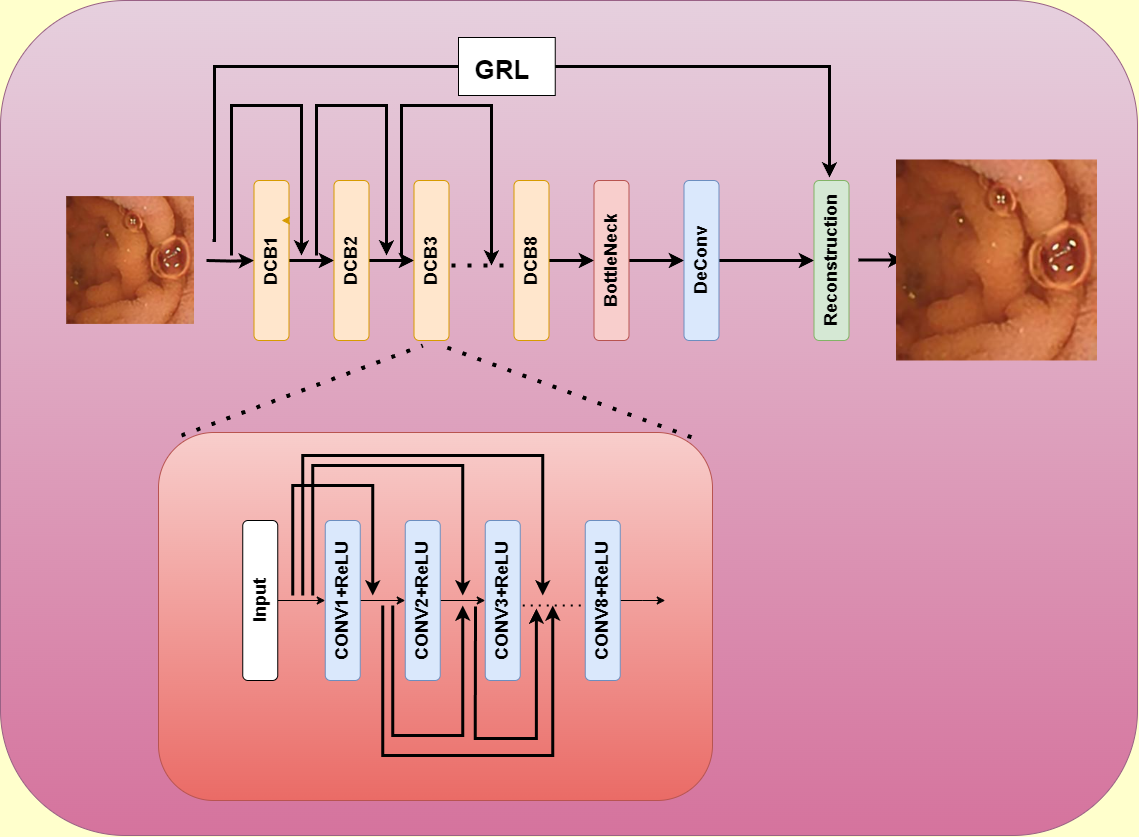
\includegraphics[totalheight=4.5in]{Chapter6/DenseGRL_UP.png}
    \caption[Upsampling Network for Dense CycleCNN]{Upsampling Network for Dense CycleCNN.}
    \label{fig:label6.4}
\end{figure}

\begin{figure}[H]
    \centering
    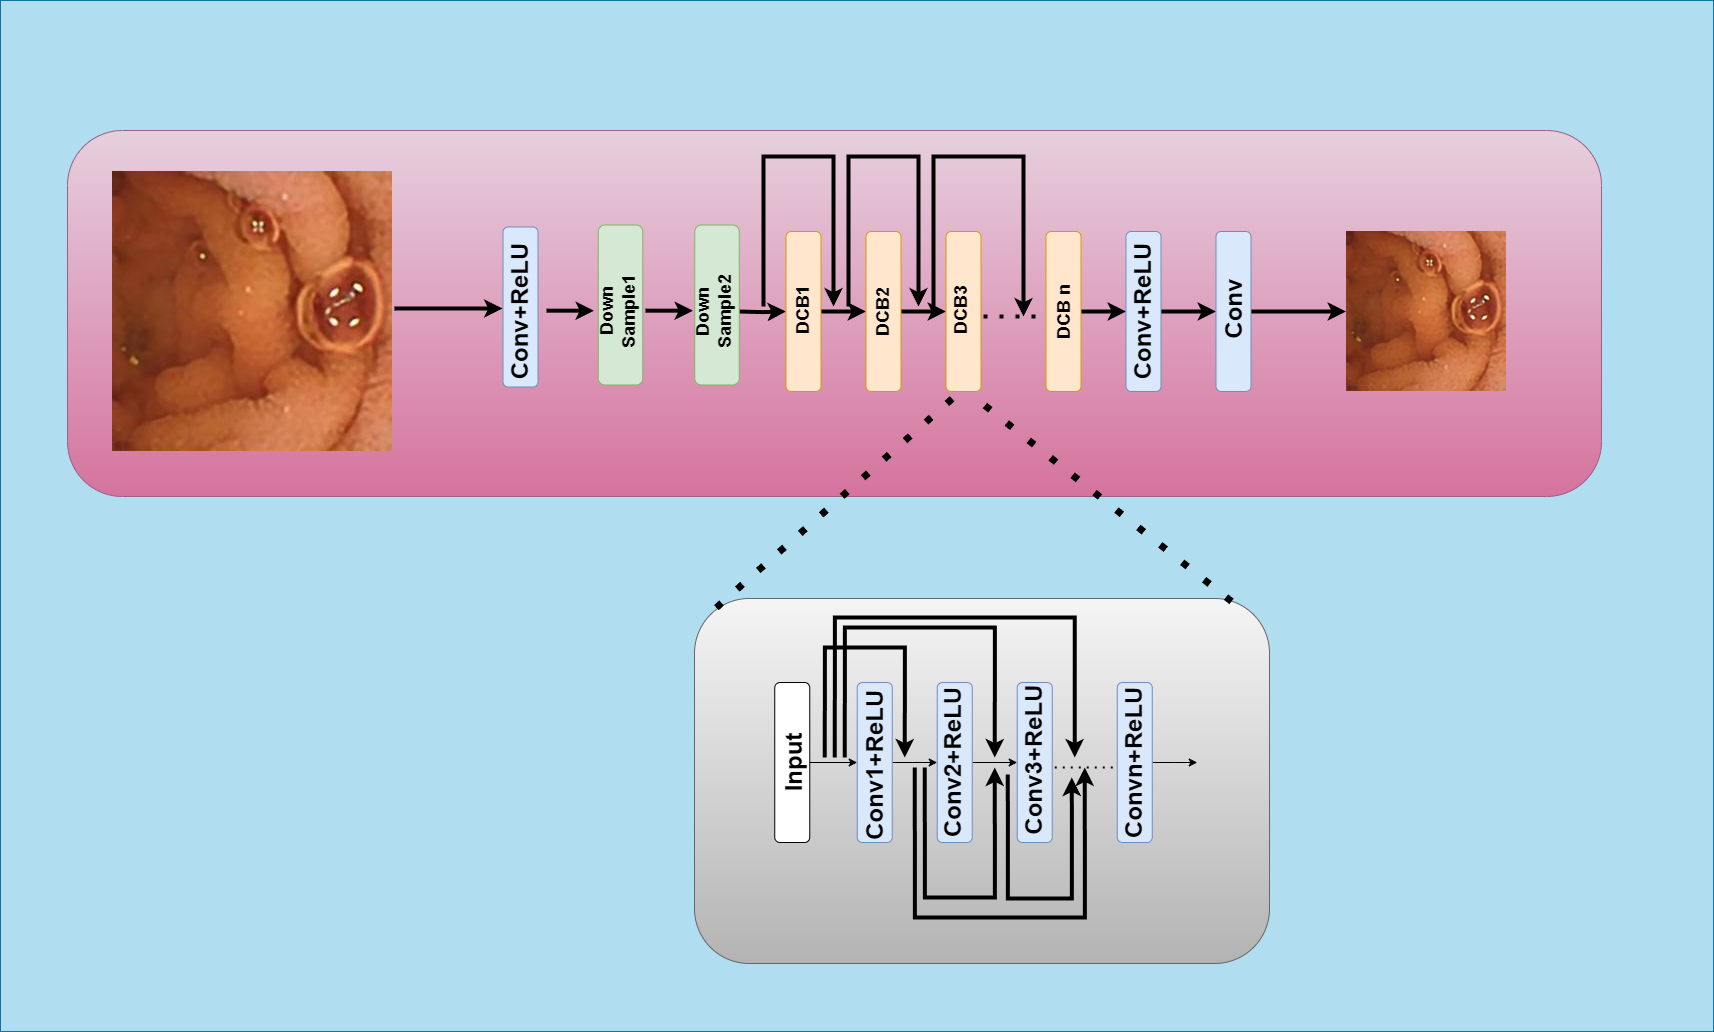
\includegraphics[totalheight=4in]{Chapter6/dense_cycle_Downsample.png}
    \caption[Downsampling Network for Dense CycleCNN]{Downsampling Network for Dense CycleCNN.}
    \label{fig:label6.6}
\end{figure}





\section{Dense CycleCNN with GRL block on YCbCr Colour space}
Due to increasing network complexity and training parameters, model training was getting very much slower, to speed up the model training we decided to train the network on Y-channel of YCbCr colour space. It has been shown in paper that the high frequency details in the image are easily captured in the Y-channel. Hence the image is first converted into from RGB colour space to YCbcr colour space and only training is done only on the Y-channel while Cb and Cr components are obtained by simple Bicubic interpolation.
\newline
The RGB components as well as the YCbCr components are shown in the Fig. \ref{fig:label6.6}
\begin{figure}[H]
    \centering

      \begin{subfigure}[b]{0.3\textwidth}
    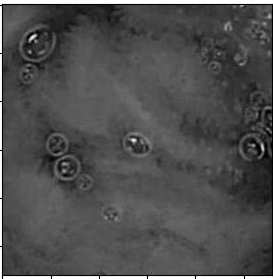
\includegraphics[width=\textwidth]{Chapter6/Blue_9.png}
    \caption{Blue Channel}
  \end{subfigure}
  \begin{subfigure}[b]{0.3\textwidth}
    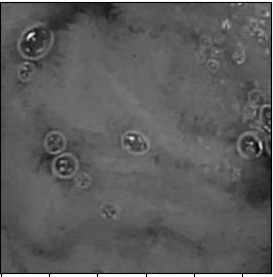
\includegraphics[width=\textwidth]{Chapter6/Green_9.png}
    \caption{Green Channel}
  \end{subfigure}
  \begin{subfigure}[b]{0.3\textwidth}
    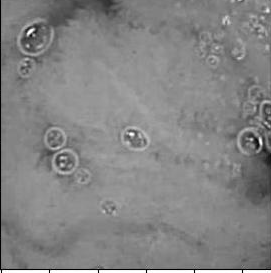
\includegraphics[width=\textwidth]{Chapter6/red_9.png}
    \caption{Red Channel}
  \end{subfigure}
  
  \begin{subfigure}[b]{0.3\textwidth}
    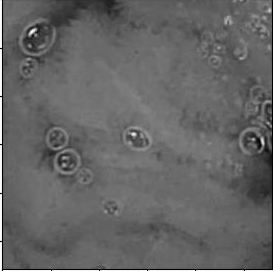
\includegraphics[width=\textwidth]{Chapter6/Y_9.png}
    \caption{Y Channel}
  \end{subfigure}
  \begin{subfigure}[b]{0.3\textwidth}
    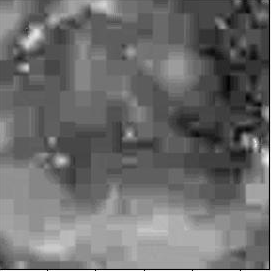
\includegraphics[width=\textwidth]{Chapter6/CB_9.png}
    \caption{Cb Channel}
  \end{subfigure}
  \begin{subfigure}[b]{0.3\textwidth}
    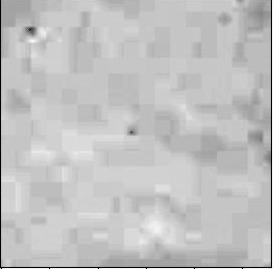
\includegraphics[width=\textwidth]{Chapter6/CR_9.png}
    \caption{Cr Channel}
  \end{subfigure}
    
    \caption[Image in different colour spaces.]{Image in different colour spaces.}
    \label{fig:label6.6}
\end{figure}
Training on Y-channel of YCbCr colour space reduces the training parameters drastically. The results obtained after training the Dense CycleCNN model on Y channel are shown in Fig. \ref{fig:label7.3}
\subsection{Dense CycleCNN with GRL Block on Patch}
Initially the training was done on whole image of 280x280. But the training was slow and it was exceeding the GPU memory. So inspired from the SRGAN \cite{SRGAN}, we did the training of the netwok on random patch of the image. The patch size taken is 100x100.
The patch training helped in training the network really fast with same results as that of training on whole image.
\newpage
\section{DenseNET with Channel Attention Block (DCAN)}
After testing various training approches and architectures mentioned above, we used the knowledge gained through these approches to design a new architecture namely DCAN-DenseNET with Channel Attention. This newtork takes into consideration the effect of Channel Attention Block(CAB) from the RCAN{\cite{RCAN}} and the idea of dense connections from SR-Densenet{\cite{DenseNET}} as they proved to be effective in capturing the high frequency details from the capsule data.


\subsection{Architecture Details}
The Channel Attention Block is used to focus the training on the important features of the image. Channel attention is able to extract the important regions of the image by exploiting the inter-channel relation of the features.

For training purpose, we have taken 8 dense blocks(i.e. num$\textunderscore $blocks=8), each consisting of 8 dense layers(num$\textunderscore$ layers=8). The number of features in consecutive dense blocks is governed by the growth rate. We have used the growth rate of 16. The number of input features and out features for the $i^{th}$ dense block is given by (growth$\textunderscore$
rate * num$\textunderscore$
layers * (i + 1), growth$\textunderscore$
rate). 
\newline
The bottle neck layer is used to compress the output features from dense connection to a lower dimension. Here, we are reducing the features to 256 features using the bottle neck layer. The deconv layer is used to upsample the images. It consist of two pixel shuffle layers each layer upsamples the image by a factor of x2. We are using pixel shuffle instead of transpose convolution because it is observed that the transpose convolution introduces the checker board effect while upsampling the image. The reconstruction layer is a convolution layer that is used to get the images number of channels that we want in our output image(i.e. num$\textunderscore$channels=3 for training on RGB channel and num$\textunderscore$channel=1 for training on Y channel of YCbCr colour space.)
The architecture of the model used is provided in the Fig.\ref{fig:label6.8}

The training is done to minimize the loss function which is the taken as the Mean Squared Loss(MSE). The training is completed for a total of 300 epochs with a batch size of 32. We did the training on patch of image, each of size 100x100, and on the Y channel of YCbCr channel. We already illustrated the benifits of training on patch of image and Y channel of YCbCr above. Adam optimizer with a learning rate of 0.0001. The quantitative analysis and qualitative analysis of the proposed model (DCAN) is shown in upcoming sections.

\begin{figure}[H]
    \centering
    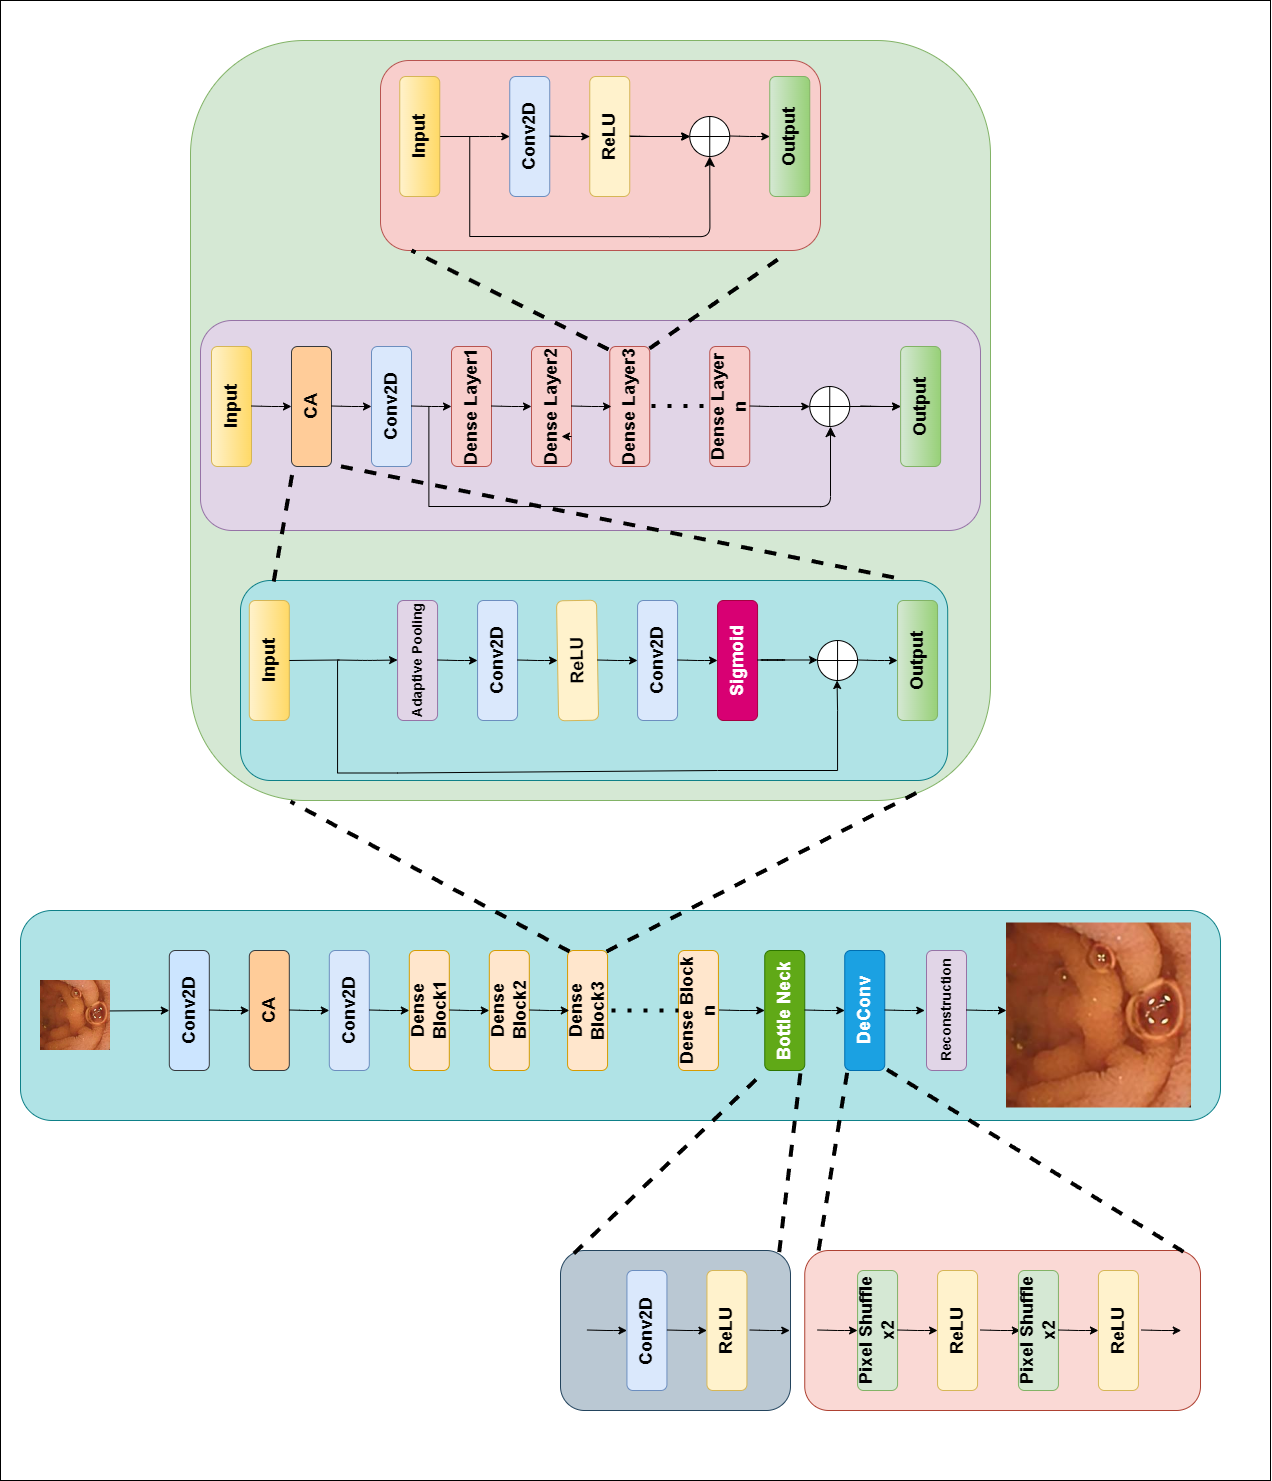
\includegraphics[totalheight=7.5in]{Chapter6/Proposed_Final.png}
    \caption[DCAN architecture]{DCAN architecture}
    \label{fig:label6.8}
\end{figure}






